\chapter{Background and theoretical framework}
\label{ch:background}

\section{Financial mathematics: option pricing}
\label{sec:financial_background}
\textcolor{red}{to be expanded: introduction}\\
In this section, we will first provide a brief introduction to the language of financial mathematics, and then introduce the Black-Scholes model for option pricing.

\subsection{Setting and options}
\textcolor{red}{change to continuous time}\\s
Let $\mathcal{T}$ be the set of trading times, and let $\Omega$ be the state space of the price of a stock. Let $\mathcal{P} = \{\mathcal{P}_t\}_{t\in\mathcal{T}}$ be a filtration on $\Omega$. On this setting, we can define a locally riskless asset $\{B(t)\}_{t\in\mathcal{T}}$, described by a $\mathcal{P}_t$-measurable stochastic process $\{r(t)\}_{t\in\mathcal{T}}$, which is the return of $B(t)$ at time $t$. The return is defined as:
\begin{equation}
    r(t) = \frac{B(t+1)-B(t)}{B(t)} \quad \forall t\in\mathcal{T}
\end{equation}
We can also define N risky assets as $\mathcal{P}_{t+1}$-measurable stochastic processes $\{S_i(t)\}_{t\in\mathcal{T}} \; i\in \{1,\dots,N\}$, which is the price of each asset at time $t$. Intuitively, the locally riskless asset is a bond, for which we know the return at time $t+1$ given the return at time $t$. The risky assets are stocks, for which we do not know the return at time $t+1$ given the return at time $t$.

% fix to make it continous time!!

% Let $\theta_j = \{\theta_j(t)\}_{t\in\mathcal{T}}$ be stochastic process representing the value of the position held in the j-th asset, which might be positive or negative (in the case of short selling).

\textcolor{red}{TBA: definition of no arbitrage}

We can now go ahead and define what a european call option is.
\begin{definition}
    A european call option is a contract that gives the holder the right, but not the obligation, to buy an asset at a specified price (the strike price) at a specified time (the expiration date). The payoff of a european call option at time $t$ is given by:
    \begin{equation}
        X(t) = \begin{cases}
            max(S(t)-K,0) & \text{if } t = T\\
            0 & \text{if } t < T
        \end{cases}
    \end{equation}
    Where $S(t)$ is the price of the underlying asset at time $t$, $K$ is the strike price, and $T$ is the expiration date. The payoff is zero if the option is not exercised, and it is equal to the difference between the price of the underlying asset and the strike price if the option is exercised.
\end{definition}

A european put option is defined similarly, as the right to sell an asset at a specified price at a specified time.

\subsection{The Black-Scholes model}
\subsubsection{Assumptions}
The Black-Scholes model is a mathematical model for the pricing of european options when $\mathcal{T}=[0,+\infty)$, introduced in \cite{black_scholes}. The assumptions for deriving the price of the option are:
\begin{enumerate}
    \item The locally riskless asset is known and constant over time: $r(t) = r \;\forall t\in\mathcal{T}$.
    \item  \label{it:gbm}The risky asset follows a geometric Brownian motion, meaning that the price of the asset at time $t$ satisfies the SDE:
    \begin{equation}
        dS(t) = \mu S(t) dt + \sigma S(t) dW(t)
    \end{equation}
    Where $W(t)$ is a standard Brownian motion, $\mu$ is the constant drift, and $\sigma$ is the volatility of the asset.
    \item The market is frictionless, meaning that there are no transaction costs, and the assets can be traded continuously.
    \item The asset pays no dividends.
    \item It is possible to short-sell the asset without any restrictions or penalties.
    \item It is possible to borrow a fraction of the security at the risk-free rate.
\end{enumerate}

\subsubsection{Derivation}
Let \( V(S,t) \) be the price of a derivative (e.g., a European call option) written on the underlying asset \( S(t) \).

Applying Itô's Lemma to \( V(S,t) \), we have:
\[
dV = \frac{\partial V}{\partial t} dt + \frac{\partial V}{\partial S} dS + \frac{1}{2} \frac{\partial^2 V}{\partial S^2} dS^2
\]

Substitute the dynamics of \( S(t) \):
\[
dS = \mu S dt + \sigma S dW
\]
\[
dS^2 = (\sigma S)^2 dt = \sigma^2 S^2 dt
\]

Thus:
\[
dV = \frac{\partial V}{\partial t} dt + \frac{\partial V}{\partial S} (\mu S dt + \sigma S dW) + \frac{1}{2} \frac{\partial^2 V}{\partial S^2} \sigma^2 S^2 dt
\]

Simplify:
\[
dV = \left( \frac{\partial V}{\partial t} + \mu S \frac{\partial V}{\partial S} + \frac{1}{2} \sigma^2 S^2 \frac{\partial^2 V}{\partial S^2} \right) dt + \sigma S \frac{\partial V}{\partial S} dW
\]

Now, construct a hedged portfolio \( \Pi = V - \Delta S \), where \( \Delta = \frac{\partial V}{\partial S} \). The change in the portfolio is:
\[
d\Pi = dV - \Delta dS
\]

Substituting:
\[
d\Pi = \left( \frac{\partial V}{\partial t} + \frac{1}{2} \sigma^2 S^2 \frac{\partial^2 V}{\partial S^2} \right) dt
\]

Note that the \( dW \) terms cancel because:
\[
\sigma S \frac{\partial V}{\partial S} dW - \frac{\partial V}{\partial S} \sigma S dW = 0
\]

This portfolio is riskless, and by the no-arbitrage assumption, it must grow at the risk-free rate:
\[
d\Pi = r \Pi dt = r(V - \Delta S) dt
\]

Equating both expressions for \( d\Pi \):
\[
\left( \frac{\partial V}{\partial t} + \frac{1}{2} \sigma^2 S^2 \frac{\partial^2 V}{\partial S^2} \right) dt = r \left( V - S \frac{\partial V}{\partial S} \right) dt
\]

Cancelling \( dt \) and rearranging terms:
\[
\frac{\partial V}{\partial t} + \frac{1}{2} \sigma^2 S^2 \frac{\partial^2 V}{\partial S^2} + r S \frac{\partial V}{\partial S} - rV = 0
\]

This is the Black-Scholes partial differential equation (PDE).

\subsubsection{Formula}

The Black-Scholes formula for a European call option with strike price \( K \), time to maturity \( T - t \), and current underlying price \( S \) is:

\[
V(S,t) = S \Phi(d_1) - K e^{-r(T - t)} \Phi(d_2)
\]

where:
\[
d_1 = \frac{\ln(S/K) + (r + \frac{1}{2} \sigma^2)(T - t)}{\sigma \sqrt{T - t}}, \quad
d_2 = d_1 - \sigma \sqrt{T - t}
\]

and \( \Phi(\cdot) \) is the cumulative distribution function of the standard normal distribution.

\subsection{Discussion}
The Black-Scholes model relies on several key assumptions, one of which is that the price of the underlying asset follows a geometric Brownian motion with constant volatility. While this assumption is mathematically convenient and allows for an analytical solution to the pricing problem, it does not always align with empirical observations of financial markets.

In practice, the distribution of asset returns often exhibits fat tails, meaning that extreme events (large positive or negative returns) occur more frequently than predicted by a normal distribution. Furthermore, returns are not always independent over time; they often exhibit autocorrelation, which violates the assumption of independent increments in the geometric Brownian motion.

These discrepancies have significant implications. For instance, the assumption of normally distributed returns can lead to an underestimation of the probability and impact of extreme market events, such as the 1987 stock market crash, the 2008 financial crisis, or the COVID-19 pandemic-induced market turmoil. Such underestimations can result in inadequate risk management strategies.

Given the widespread use of the Black-Scholes model and its extensions in the financial industry, particularly in the pricing of derivatives, understanding the limitations of its assumptions is crucial. According to \cite{bis}, the notional value of the over-the-counter derivatives market has reached approximately \$730 trillion. This highlights the potential global impact of mispricing and underestimating risks due to unrealistic assumptions.

To address these limitations, alternative models have been proposed that aim to capture more realistic dynamics of asset prices. One promising approach is to model price movements based on the interplay of supply and demand, which is driven by the collective behavior of market participants. This perspective naturally leads to the study of models inspired by statistical physics, where the interactions of many agents are explicitly considered. In the next section, we will introduce key concepts from statistical physics to formalize this approach.


\section{Statistical physics: the Ising model}
In this section, we introduce the Ising model as an example of model driven by the interaction of many agents (spins). The Ising model is a simple mathematical model of ferromagnetic materials. In its description, we will mostly follow the notation and tools presented in \cite{mezard_book} and from professor Mézard's lecture notes. The model consists of Ising spins (that is, spins which can take binary values) on a d-dimensional cubic lattice (see figure \ref{fig:ising_model}). Mathematically, given a cubic lattice $\mathbb{L}=\{1,\dots,L\}^n$, we define an an Ising spin $\sigma_i\in\{-1,1\}$ for each site $i\in\mathbb{L}$. Then, we can have any configuration $\underline{\sigma} = (\sigma_1,\dots,\sigma_n) \in \mathcal{X}_N=\{+1,-1\}^{\mathbb{L}}$.

\begin{figure}[h]
    \centering
    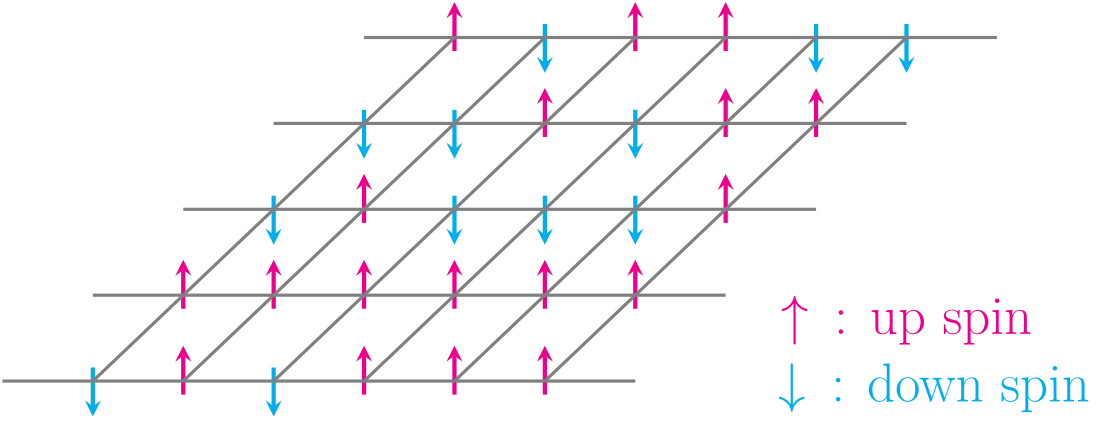
\includegraphics[width=0.5\textwidth]{2D_ising_model_on_lattice.svg.png}
    \caption{The Ising model on a 2D lattice.}
    \label{fig:ising_model}
\end{figure}


The energy of a configuration $\underline{\sigma}$ is given by:
\begin{equation}
    H(\underline{\sigma}) = -\sum_{\langle i,j\rangle}\sigma_i\sigma_j - B\sum_i \sigma_i
\end{equation}
Where the sum over $\langle i,j\rangle$ is a sum over all nearest neighbors, and $B$ is an external magnetic field. At equilibrium, the probability of a configuration $\underline{\sigma}$ is given by the Boltzmann distribution:
\begin{equation}
    P(\underline{\sigma}) = \frac{e^{-\beta H(\underline{\sigma})}}{Z}
\end{equation}
Where $\beta$ is the inverse temperature, and $Z$ is the partition function:
\begin{equation}
    Z = \sum_{\underline{\sigma}\in\mathcal{X}_N}e^{-\beta H(\underline{\sigma})}
\end{equation}
Interestingly, despite its simplicity, an analytical, closed-form solution for \(Z\) has been found only in the $d=1$ and $d=2$ cases. Higher dimensions remain unsolved, but numerical methods and mean-field approximations can be used to study the model in these cases.

One important quantity in the Ising model is the magnetization, which is defined as:
\begin{equation}
    m = \frac{1}{N}\sum_i \langle \sigma_i \rangle
\end{equation}
where $\langle \cdot \rangle$ denotes the average.

\subsection{Solution of the Ising model in the one-dimensional case}
For simplicity, assume $B=0$. In the one-dimensional case, the Ising model can be solved exactly. Recall that:
\begin{equation}
    H(\underline{\sigma}) = -\sum_{\langle i,j\rangle}\sigma_i\sigma_j
\end{equation}
Then, the partition function is given by:
\begin{equation}
    Z = \sum_{\underline{\sigma}\in\mathcal{X}_N}e^{-\beta H(\underline{\sigma})} =
    \sum_{\underline{\sigma}\in\mathcal{X}_N}e^{\beta\sum_{\langle i,j\rangle}\sigma_i\sigma_j}
\end{equation}
Since each spin is connected to its nearest neighbors, we can write:
\begin{equation}
    Z =  \sum_{\underline{\sigma}\in\mathcal{X}_N}e^{\beta\sum_n\sigma_n\sigma_{n+1}}
\end{equation}
Let us define $\tau_n = \sigma_{n-1}\sigma_{n} \implies \sigma_n = \tau_n\tau_{n-1}\dots\tau_2\sigma_1$. Then, we can write:
\begin{equation}
    \begin{gathered}
    Z =  \sum_{\sigma_1\in\{-1,1\}}\sum_{\tau_2,\dots\tau_n}e^{\beta\sum_n\tau_n}
    = 2\sum_{\tau_2,\dots,\tau_N}e^{\beta\sum_n\tau_n}\\
    = 2\sum_{\tau_2,\dots,\tau_N}\prod_n e^{\beta\tau_n}
    = 2(\sum_{\tau_2}e^{\beta\tau_2})\dots(\sum_{\tau_N}e^{\beta\tau_N})\\
    = 2(2\cosh(\beta))^{N}
    \end{gathered}
\end{equation}
Thus, we have found an analytical expression for the partition function in the one-dimensional case. The magnetization can be computed as:
\begin{equation}
    m = \frac{1}{N}\sum_i \langle \sigma_i \rangle = \frac{1}{N}\frac{\partial}{\partial \beta}\log Z = \tanh(\beta)
\end{equation}
%check magnetization formula

% \subsection{The Curie-Weiss model}
% The Curie-Weiss model is remarkably similar to the Ising model, but with all the spins interacting with each other, then, the model represents a fully connected graph of spins rather than a lattice. The Hamiltonian is given by:
% \begin{equation}
%     H(\underline{\sigma}) = -\frac{1}{N}\sum_{i,j}\sigma_i\sigma_j - B\sum_i \sigma_i
% \end{equation}
% The scaling factor $\frac{1}{N}$ is introduced to have a non-trivial free energy. This model is interesting because it introduced the concept of mean-field approximations. To compute the partition function, we first notice that the empirical magnetization is:
% \begin{equation}
%     m(\underline{\sigma}) = \frac{1}{N}\sum_i  \sigma_i
% \end{equation}
% Then, we can write:
% \begin{equation}
%     H(\underline{\sigma}) = \frac{1}{2}N- \frac{1}{2}N m(\underline{\sigma})^2 - NB m(\underline{\sigma})
% \end{equation}




\subsection{Mean-field approximation of the Ising model in higher dimensions}
While a closed-form solution for the Ising model in two dimensions exists, it does not for $d\geq 3$ so we will study its mean-field approximation. The method we will see can be applied to a more general Ising model, and then be reconduced to the original one. The hamiltonian we focus on is:
\begin{equation}
    H(\underline{\sigma}) = -\sum_{\langle i,j\rangle}J_{i,j}\sigma_i\sigma_j - \sum_i B_i\sigma_i
\end{equation}
Which differs from the standard Ising model by having arbitrary $J_{i,j}$ and $B_i$ for every $i,j$. The idea is to approzimate the Boltzmann distribution $P(\underline{\sigma}) = (1/Z)e^{-\beta H(\underline{\sigma})}$ with a probability with independent variables $Q(\underline{\sigma})= \prod_{i=1}^Nq_i(\sigma_i)$. The idea is to find the $q_i$ such that the ``distance'' between $P$ and $Q$ is minimized. We will use the Kullback-Leibler divergence as notion of distance.
\begin{definition}
    Given $p(x)$ and $q(x)$ probability distributions over the same finite space $\mathcal{X}$, the Kullback–Leibler (KL) divergence between them is:
    $$D(q||p) = \sum_{x\in\mathcal{X}}q(x)\log\frac{q(x)}{p(x)}$$
\end{definition}
\begin{remark}
    \hfill
    \begin{enumerate}
        \item $D(q||p)$ is convex in $q(x)$.
        \item $D(q||p)\geq 0$ with equality $ \iff p(x)=q(x) \;\forall x\in\mathcal{X}$.
        \item In general, the KL divergence is not symmetric.
    \end{enumerate}
    Then, the KL divergence lacks the symmetry property to be properly defined as a distance between probability distributions.
\end{remark}
We will define $Q$ as the most general joint binary probability distribution:
\begin{equation}
    Q(\underline{\sigma}) = \prod_{i=1}^{N}q_i(\sigma_i); \quad
    q_i(\sigma_i)=\frac{1+m_i\sigma_i}{2}
\end{equation}
Where $m_i$ is the mean of each $q_i$, and it is the parameter which we want to find. Then,
\begin{equation}
    \begin{gathered}
        D(Q||P) = \sum_{\underline{\sigma}\in\mathcal{X}}Q(\underline{\sigma})\log\frac{Q(\underline{\sigma})}{P(\underline{\sigma})}\\
        =\sum_{\underline{\sigma}\in\mathcal{X}}Q(\underline{\sigma})\log Q(\underline{\sigma}) - \sum_{\underline{\sigma}\in\mathcal{X}}Q(\underline{\sigma})\log P(\underline{\sigma}) = (A) + (B)\\
    \end{gathered}
\end{equation}
We can split this in the first term, depending only on $Q$, and the second term, depending on $P$ as well. Then:
\begin{equation}
    \begin{gathered}
        (A) = \sum_{\underline{\sigma}\in\mathcal{X}}Q(\underline{\sigma})\log Q(\underline{\sigma}) = \sum_{i=1}^{N}\left(\frac{1+m_i}{2} \log \frac{1+m_i}{2}+\frac{1-m_i}{2} \log \frac{1-m_i}{2}\right)\\
        (B) = \beta \sum_{i<j} J_{i j} m_i m_j + \beta \sum_i B_i m_i-\log Z
    \end{gathered}
\end{equation}
In the second term, we see that the $\log Z$ term is independent of $m_i$, so we can ignore it. Then, we are interested in finding the values of $m_i$ that solve:
\begin{equation}
    \frac{\partial D(Q||P)}{\partial m_i} = 0 \iff \frac{1}{2} \log \frac{1+m_i}{1-m_i} - \beta \sum_{j\in \partial_i} J_{i j} m_j - \beta B_i = 0
\end{equation}
Then, we find the mean field equation:
\begin{equation}
    m_i = \tanh\left(\beta\sum_{j\in \partial_i} J_{i j} m_j + \beta B_i\right)
\end{equation}
Now, going back to the original Ising model, we can set $J_{i,j} = J$ and $B_i=B \implies m_i = m$. Then, we have the mean field equation for the Ising model in $d$ dimensions:
\begin{equation}
    m = \tanh(\beta (B + 2dJm))
\end{equation}
Let us consider the case $B=0$. Then, depending on the value of $\beta$, we can have one or three solutions to the mean-field equation, depending on the slope of the function $f(m) = \tanh(\beta 2dJm)$. The critical value of $\beta$ is then:
\begin{equation}
    \beta_c = \frac{1}{2dJ}
\end{equation}

\subsection{The Curie-Weiss model}
The Curie-Weiss model is a generalization of the Ising model, where instead of interacting with nearest neighbors, each spin interacts with all other spins. The Hamiltonian is given by:
\begin{equation}
    H(\underline{\sigma}) = -\frac{J}{N}\sum_{i<j}\sigma_i\sigma_j - B\sum_i \sigma_i
\end{equation}
The scaling factor $\frac{1}{N}$ is introduced to have a non-trivial free energy. This model is interesting because it introduced the concept of mean-field approximations. As usual, the partition function is given by:
\begin{equation}
    \begin{aligned}
        Z &= \sum_{\underline{\sigma}\in\mathcal{X}_N}e^{-\beta H(\underline{\sigma})}\\
        &= \sum_{\underline{\sigma}\in\mathcal{X}_N}e^{\beta\frac{J}{N}\sum_{i<j}\sigma_i\sigma_j+\beta B \sum_i \sigma_i}\\
        &= \sum_{\underline{\sigma}\in\mathcal{X}_N}e^{\frac{1}{2}\beta\frac{J}{N}\sum_{i,j}\sigma_i\sigma_j+\beta B \sum_i \sigma_i-\frac{1}{2}\beta J}\\
        &= \sum_{\underline{\sigma}\in\mathcal{X}_N}e^{\frac{1}{2}\beta\frac{J}{N}\left(\sum_{i}\sigma_i\right)^2+\beta B \sum_i \sigma_i-\frac{1}{2}\beta J}\\
    \end{aligned}
\end{equation}
Now, we can apply the Hubbard-Stratonovich transformation:
\begin{equation}
    e^{\frac{b^2}{2a}} = \int_{-\infty}^{+\infty}\frac{dx}{\sqrt{2\pi/ a}} e^{-\frac{1}{2}ax^2+bx}
\end{equation}
Then, we can rewrite the quadratic term:
\begin{equation}
    e^{\frac{1}{2}\beta\frac{J}{N}\left(\sum_{i}\sigma_i\right)^2} = \int_{-\infty}^{+\infty}\frac{dx}{\sqrt{2\pi/N}} e^{-\frac{1}{2}Nx^2+\sqrt{\beta J}\left(\sum_i \sigma_i\right)x}
\end{equation}
Then, the partition function becomes:
\begin{equation}
    \begin{aligned}
        Z &= \sum_{\underline{\sigma}\in\mathcal{X}_N}\int_{-\infty}^{+\infty}\frac{dx}{\sqrt{2\pi/N}} e^{-\frac{1}{2}Nx^2+\sqrt{\beta J}\left(\sum_i \sigma_i\right)x+\beta B \sum_i \sigma_i-\frac{1}{2}\beta J} \\
        &\approx \sum_{\underline{\sigma}\in\mathcal{X}_N}\int_{-\infty}^{+\infty}dx e^{-\frac{1}{2}Nx^2+\sqrt{\beta J}\left(\sum_i \sigma_i\right)x+\beta B \sum_i \sigma_i} \\
        &= \int_{-\infty}^{+\infty}dx e^{-\frac{1}{2}Nx^2} \sum_{\underline{\sigma}\in\mathcal{X}_N}e^{\sqrt{\beta J}\left(\sum_i \sigma_i\right)x+\beta B \sum_i \sigma_i-\frac{1}{2}\beta J}\\
        &= \int_{-\infty}^{+\infty}dx e^{-\frac{1}{2}Nx^2} \left(\sum_{\sigma \in \{-1,1\}}e^{\sqrt{\beta J}\sigma x+\beta B \sigma}\right)^N\\
        &=  \int_{-\infty}^{+\infty}dx e^{-\frac{1}{2}Nx^2+N\log\left(2\cosh(x\sqrt{\beta J}+\beta B)\right)}
    \end{aligned}
\end{equation}
Where the first approximation comes from the thermodynamic limit, where we only focus on terms which are $O(N)$ and ignore subleading terms in the exponential. Now, we can use the Laplace method to compute the integral:
\begin{equation}
    \begin{aligned}
        \int_{-\infty}^{+\infty}dx e^{Nf(x)} \approx \sqrt{\frac{2\pi}{Nf''(x_0)}}e^{Nf(x_0)}\\
    \end{aligned}
\end{equation}
Where $x_0$ is the maximum of $f(x)$, and $f''(x_0)$ is the second derivative of $f(x)$ at $x_0$. In our case:
\begin{equation}
    x_0 = \sqrt{\beta J}\tanh(x_0\sqrt{\beta J}+\beta B)
\end{equation}
Giving us an approximate solution for the partition function:
\begin{equation}
    Z \approx \sqrt{\frac{2\pi}{Nf''(x_0)}}e^{Nf(x_0)}
\end{equation}
From which we can derive the magnetization:
\begin{equation}
    m = \tanh(\beta(B+Jm))
\end{equation}
Which is the mean-field equation for the Curie-Weiss model.